\documentclass[10pt,letterpaper]{article}
\usepackage[margin=0.74in,headheight=15pt]{geometry}
\usepackage[T1]{fontenc}
\usepackage{lmodern}
\usepackage{microtype}
\usepackage{graphicx}
\usepackage{xurl}
\usepackage{booktabs,tabularx,array}
\usepackage{enumitem}
\usepackage{xcolor}
\usepackage{tikz}
\usetikzlibrary{arrows.meta,positioning,calc,fit,backgrounds,decorations.pathreplacing}
\usepackage{pgfplots}
\pgfplotsset{compat=1.18,unbounded coords=jump}
\usepackage{fancyhdr}
\usepackage{hyperref}
\usepackage{bookmark}
\hypersetup{colorlinks=true,linkcolor=blue!45!black,urlcolor=blue!45!black}
\definecolor{ink}{RGB}{32,48,67}
\definecolor{blue}{RGB}{0,108,162}
\definecolor{green}{RGB}{35,133,91}
\definecolor{orange}{RGB}{202,110,37}
\definecolor{red}{RGB}{201,78,78}
\definecolor{papergray}{RGB}{243,245,247}
\newcommand{\key}[1]{\textbf{#1}}
\newcommand{\sourcefile}[1]{\par\smallskip{\footnotesize\color{ink}\textit{Source checked: }\url{#1}.}\par}
\newcommand{\teachingnote}[1]{\begin{center}\begin{minipage}{.88\linewidth}\colorbox{papergray}{\parbox{.94\linewidth}{\small\textbf{A useful way to read this:} #1}}\end{minipage}\end{center}}
\pagestyle{fancy}
\fancyhf{}
\lhead{A plain-language guide to safe antenna motion}
\rhead{\thepage}
\setlength{\parskip}{0.52em}
\setlength{\parindent}{0pt}
\begin{document}
\pagenumbering{gobble}
\begin{titlepage}
\centering
\vspace*{1.1in}
{\Huge\bfseries How the Antenna Finds a Safe Way to Turn\par}
\vspace{.35in}
{\Large A picture-led guide to the motion planner\par}
\vfill
\begin{minipage}{.82\textwidth}
\large
An antenna can point in many directions, but not every direction is safe.
This guide shows how the software chooses a route, turns it into a real
movement, and checks the answer independently before calling it successful.
It is written for a curious reader, not an engineer.
\end{minipage}
\vfill
\large Current-source edition, rebuilt from the planner in this worktree
\end{titlepage}
\pagenumbering{arabic}
\tableofcontents
\clearpage

\section{The machine and the map}

Think of the antenna as a camera on a two-way hinge. One angle turns it left or
right; the other tips it up or down. The software calls them \key{azimuth} and
\key{elevation}. For planning, it lays those two angles flat on a map. A dot on
the map is one direction the antenna can face.

The task is simple to say: start at the blue dot, finish at the green dot, and
never point through the red blocked area. The red area includes a small safety
buffer, so getting close is treated as unsafe too. This is a map of directions,
not a floor plan the antenna travels across.

\begin{figure}[ht]
\centering
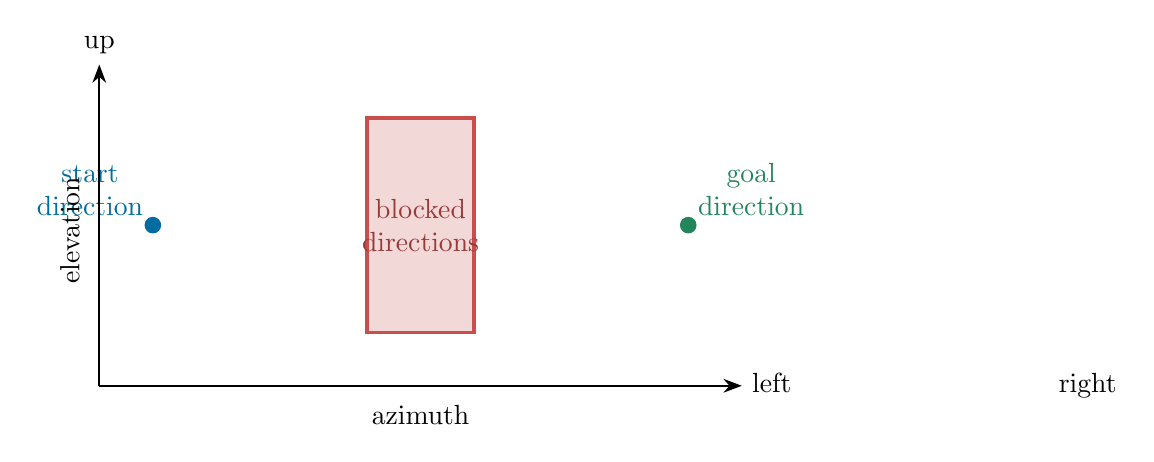
\begin{tikzpicture}[x=.68cm,y=.68cm,>=Stealth]
\fill[red!22] (-1,-2) rectangle (1,2);
\draw[red,very thick] (-1,-2) rectangle (1,2);
\fill[blue] (-5,0) circle (3pt) node[above left,align=center]{start\\direction};
\fill[green] (5,0) circle (3pt) node[above right,align=center]{goal\\direction};
\node[align=center,text=red!75!black] at (0,0){blocked\\directions};
\draw[->,thick] (-6,-3)--(6,-3) node[right]{left \hspace{9em} right};
\draw[->,thick] (-6,-3)--(-6,3) node[above]{up};
\node[rotate=90] at (-6.55,-.1){elevation};
\node at (0,-3.55){azimuth};
\end{tikzpicture}
\caption{One direction is one place on the flat azimuth--elevation map.}
\label{fig:map}
\end{figure}

\teachingnote{The picture has deliberately flattened the problem. It lets us see
the direction choices before we talk about time or speed.}

\section{Why drawing a line is not enough}

The most direct mark between the two dots is a straight line. It fails: part of
it cuts through a blocked direction. The working route bends around the area
instead. That first lesson is important: a route is not judged by how neat it
looks, but by whether every part of it stays out of the blocked region.

\begin{figure}[ht]
\centering
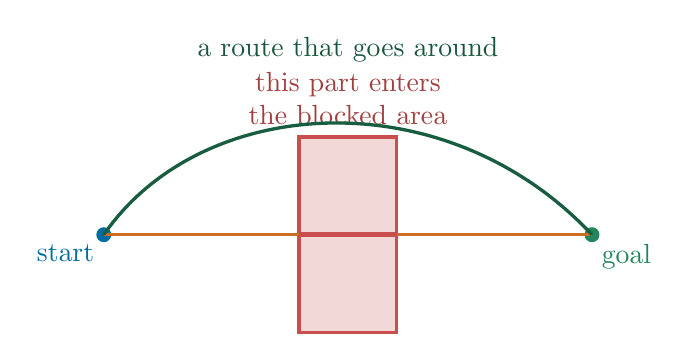
\begin{tikzpicture}[x=.62cm,y=.62cm,>=Stealth]
\fill[red!22] (-1,-2) rectangle (1,2);
\draw[red,very thick] (-1,-2) rectangle (1,2);
\fill[blue] (-5,0) circle (2.7pt) node[below left]{start};
\fill[green] (5,0) circle (2.7pt) node[below right]{goal};
\draw[orange,very thick] (-5,0)--(5,0);
\draw[red,ultra thick] (-1,0)--(1,0);
\node[text=red!80!black,align=center] at (0,2.8){this part enters\\the blocked area};
\draw[green!70!black,very thick] (-5,0) .. controls (-3,2.9) and (2,3.2) .. (5,0);
\node[text=green!65!black,align=center] at (0,3.8){a route that goes around};
\end{tikzpicture}
\caption{The broken rule and the working alternative, shown together.}
\label{fig:line}
\end{figure}

The route in this picture is still only a suggestion. It does not yet say how
fast the antenna moves, whether it can make the bend smoothly, or whether the
whole movement is safe between the few points we drew. Those are the harder
parts of the job.

\clearpage

\section{Turning a route into a movement}

The curve on the map tells us \emph{where} the antenna should point. It still
does not tell us \emph{when}. A useful way to make time visible is to place a
dot on the real motion every half second. Dots close together mean the antenna
covered little ground during that half second. Dots far apart mean it covered
more ground.

Figure~\ref{fig:timedmotion} comes from an actual successful run of the
maintained obstacle example. The small blue dots are equal half-second moments,
not extra route choices. The antenna starts gently because it is still building
up speed. It later travels faster, then slows to arrive without a jolt.

\begin{figure}[p]
\centering
\begin{tikzpicture}
\begin{axis}[width=.92\textwidth,height=.54\textwidth,axis equal image,
xlabel={azimuth (degrees)},ylabel={elevation (degrees)},
xmin=-5.8,xmax=5.8,ymin=-2.8,ymax=3.25,grid=major,
legend style={at={(.5,-.19)},anchor=north,legend columns=3,font=\scriptsize}]
\addplot[fill=red!20,draw=red,very thick] table[x index=0,y index=1,
col sep=tab]{data/protected_obstacle.dat} \closedcycle;
\addlegendentry{blocked directions plus safety buffer}
\addplot[blue,very thick,mark=none] table[x index=1,y index=2,
col sep=tab]{data/selected_motion.dat};
\addlegendentry{real smooth motion}
\addplot[only marks,blue,mark=*,mark size=1.6pt] table[x index=1,y index=2,
col sep=tab]{data/half_second_motion.dat};
\addlegendentry{one dot every half second}
\addplot[only marks,mark=*,mark size=2.2pt,blue] coordinates {(-5,0)};
\addplot[only marks,mark=*,mark size=2.2pt,green] coordinates {(5,0)};
\node[fill=white,draw=blue,rounded corners,align=left,font=\scriptsize] at
(axis cs:-3.8,2.65){slow here:\\still speeding up};
\draw[->,blue,thick] (axis cs:-3.45,2.35) -- (axis cs:-4.45,.58);
\node[fill=white,draw=green!70!black,rounded corners,align=left,font=\scriptsize] at
(axis cs:.8,3.0){fast here};
\draw[->,green!70!black,thick] (axis cs:.55,2.75) -- (axis cs:.35,2.43);
\end{axis}
\end{tikzpicture}
\caption{Time made visible. The dot spacing comes from the exported successful
motion; no dots were moved to make the picture look smoother.}
\label{fig:timedmotion}
\end{figure}

The antenna also has limits. It cannot turn a direction angle as quickly as it
likes, and it cannot suddenly change from slow to fast. The planner keeps track
of the turning speed, the change of that speed, and the change of that change.
The last two are the practical reason a sharp-looking corner on a map may be
impossible for a real machine to follow.

\begin{figure}[ht]
\centering
\begin{tikzpicture}
\begin{axis}[width=.91\textwidth,height=.43\textwidth,
xlabel={time (seconds)},ylabel={fastest coordinate speed (degrees per second)},
xmin=0,xmax=7.7,ymin=0,ymax=2.25,grid=major,
legend style={at={(.5,-.2)},anchor=north,legend columns=2,font=\scriptsize}]
\addplot[blue,very thick,mark=none] table[x index=0,y index=1,
col sep=tab]{data/turning_speed.dat};
\addlegendentry{real motion}
\addplot[red,densely dashed,very thick] coordinates {(0,2) (7.7,2)};
\addlegendentry{allowed maximum: 2}
\addplot[only marks,mark=*,mark size=2.3pt,orange] coordinates {(3.55,1.9869)};
\node[fill=white,draw=orange,rounded corners,align=left,font=\scriptsize] at
(axis cs:5.25,1.42){closest approach: 1.9869\\still below the 2.0 limit};
\draw[->,orange,thick] (axis cs:4.45,1.55)--(axis cs:3.55,1.9869);
\end{axis}
\end{tikzpicture}
\caption{A real limit, shown with real numbers. In this run the motion comes
within 0.0131 degrees per second of the limit; it does not claim to touch it.}
\label{fig:speed}
\end{figure}

\teachingnote{A limit is not a target. Going faster would be attractive only if
the machine could still stay within every limit and avoid every blocked direction.}

\clearpage

\section{How the software gets a route to try}

The program first draws several possible straight pieces between useful points:
the start, the goal, and places on the edge of the blocked region. These pieces
are \key{candidates}: ideas worth trying, not approved answers. It can reject a
piece immediately when it enters a blocked area. It can keep a piece that stays
outside, while still rejecting the full route later if a smooth movement cannot
be made along it.

In Figure~\ref{fig:candidates}, faint gray marks show the real candidate pieces
considered in the same successful example. The two bold pieces are the lesson:
one passes through the protected rectangle and is rejected; the other stays
outside it and is allowed to remain a suggestion.

\begin{figure}[p]
\centering
\begin{tikzpicture}
\begin{axis}[width=.92\textwidth,height=.56\textwidth,axis equal image,
xlabel={azimuth (degrees)},ylabel={elevation (degrees)},
xmin=-5.8,xmax=5.8,ymin=-2.9,ymax=3.1,grid=major]
\addplot[gray!50,thin,mark=none] table[x index=0,y index=1,
col sep=tab]{data/visibility_accepted_segments.dat};
\addplot[gray!50,thin,mark=none] table[x index=0,y index=1,
col sep=tab]{data/visibility_rejected_segments.dat};
\addplot[fill=red!20,draw=red,very thick] table[x index=0,y index=1,
col sep=tab]{data/protected_obstacle.dat} \closedcycle;
\addplot[orange,very thick,mark=none] table[x index=0,y index=1,
col sep=tab]{data/rejected_direct_line.dat};
\addplot[green!70!black,very thick,mark=none] table[x index=0,y index=1,
col sep=tab]{data/allowed_candidate_line.dat};
\addplot[only marks,mark=*,mark size=2.2pt,blue] coordinates {(-5,0)};
\addplot[only marks,mark=*,mark size=2.2pt,green] coordinates {(5,0)};
\node[fill=white,draw=orange,rounded corners,align=left,font=\scriptsize] at
(axis cs:-2.8,-1.2){rejected:\\it passes through};
\draw[->,orange,thick] (axis cs:-2.45,-1.0)--(axis cs:-.25,-.05);
\node[fill=white,draw=green!70!black,rounded corners,align=left,font=\scriptsize] at
(axis cs:3.15,-2.45){allowed:\\it stays outside};
\draw[->,green!70!black,thick] (axis cs:2.7,-2.15)--(axis cs:1.1,-2.2);
\end{axis}
\end{tikzpicture}
\caption{One clear allowed piece and one clear rejected piece, with the rest of
the real candidate lines faded into the background.}
\label{fig:candidates}
\end{figure}

The planner records what it tried. If none of the proposed routes leads to a
movement that passes the final check, it returns an honest ``no safe motion was
found'' result together with the evidence of its search. That is different from
saying no safe motion could possibly exist.

\clearpage

\section{How the software checks the safe side}

A curve that looks clear in a picture still needs a stronger check. The planner
uses a simple idea that can be drawn as a \key{safety line}. For one small part
of the path, it tries to put a straight line between that part and the blocked
region. The path stays entirely on one side; the blocked region stays entirely
on the other. The line is a witness that the two are separated.

The important word is \emph{entirely}. If the path has already entered the
blocked region, no separating line can be put between them. The program must
then change the proposed motion and try again. It does not erase the bad part
or quietly push the final answer out of the way.

\begin{figure}[ht]
\centering
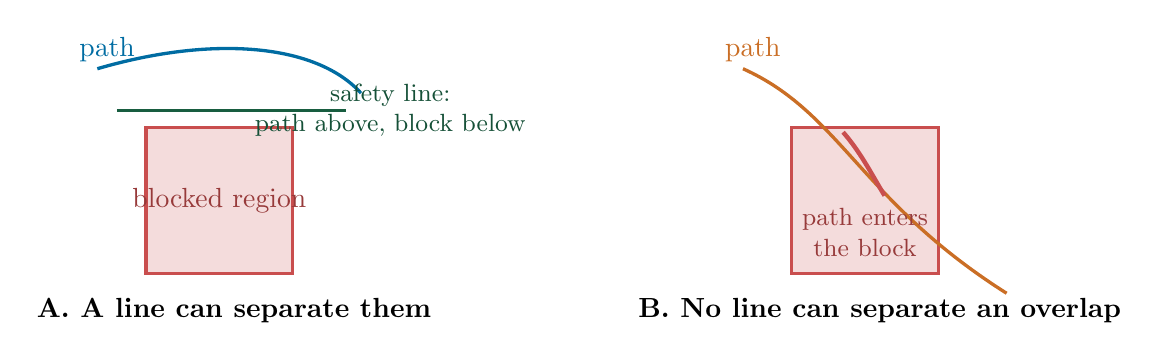
\begin{tikzpicture}[x=.62cm,y=.62cm,>=Stealth]
\begin{scope}
\fill[red!20] (0,0) rectangle (3,3);
\draw[red,very thick] (0,0) rectangle (3,3);
\draw[blue,very thick] (-1,4.2) .. controls (1.4,4.9) and (3.5,4.7) .. (4.4,3.7);
\draw[green!70!black,very thick] (-.6,3.35)--(4.1,3.35);
\node[text=green!60!black,align=center,font=\small] at (5.0,3.35){safety line:\\path above, block below};
\node[text=red!75!black] at (1.5,1.5){blocked region};
\node[text=blue] at (-.8,4.6){path};
\node[font=\bfseries] at (1.8,-.75){A. A line can separate them};
\end{scope}
\begin{scope}[xshift=8.2cm]
\fill[red!20] (0,0) rectangle (3,3);
\draw[red,very thick] (0,0) rectangle (3,3);
\draw[orange,very thick] (-1,4.2) .. controls (1.0,3.3) and (1.4,1.5) .. (4.4,-.4);
\draw[red,ultra thick] (1.05,2.9) .. controls (1.4,2.5) and (1.6,2.1) .. (1.9,1.6);
\node[text=red!75!black,align=center,font=\small] at (1.5,.85){path enters\\the block};
\node[text=orange] at (-.8,4.6){path};
\node[font=\bfseries] at (1.8,-.75){B. No line can separate an overlap};
\end{scope}
\end{tikzpicture}
\caption{The safety-line idea. The real engine uses this idea repeatedly for
small spans of a smooth motion and the protected obstacle regions.}
\label{fig:safetyline}
\end{figure}

This check is stronger than taking a few snapshots. A quick snapshot might miss
the moment between two samples when a moving antenna cuts a corner. The final
check examines the complete smooth pieces of the motion. A result is successful
only after that separate check passes.

\section{Why it repeats}

One attempt is rarely enough. The program makes a smooth movement for a
candidate route, looks for any places where the movement and blocked region are
not separated, improves the safety lines, and tries another movement. It keeps
the best safe motion it has seen while it works.

The next picture is deliberately candid about what the current record contains.
The engine records each attempt's arrival time, whether it was clear, and how
many path--block pairs still overlapped. It does \emph{not} save the full
coordinates of every intermediate attempt. The three curves below therefore
illustrate the visible correction, while their time labels and safe/unsafe
status are the real records from the exported run.

\begin{figure}[p]
\centering
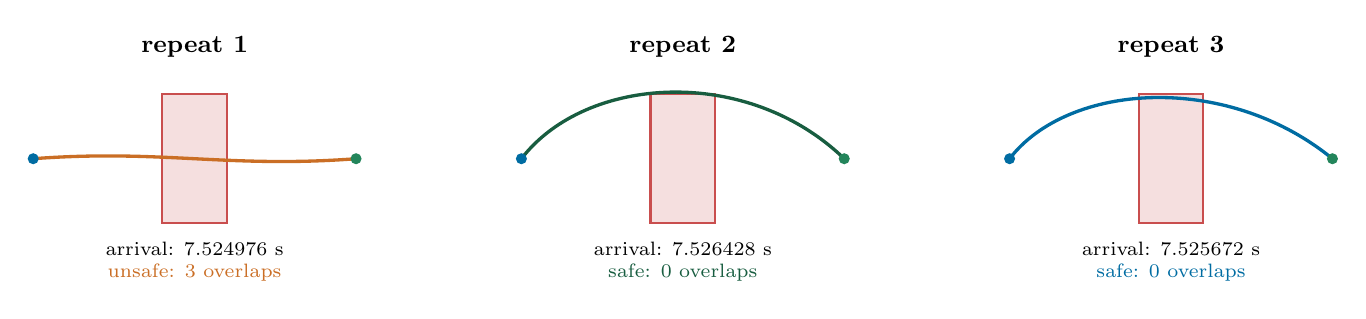
\begin{tikzpicture}[x=.41cm,y=.41cm]
\begin{scope}
\fill[red!18] (-1,-2) rectangle (1,2); \draw[red,thick] (-1,-2) rectangle (1,2);
\draw[orange,very thick] (-5,0) .. controls (-1,.3) and (1,-.3) .. (5,0);
\fill[blue] (-5,0) circle (2pt); \fill[green] (5,0) circle (2pt);
\node[align=center,font=\small\bfseries] at (0,3.45){repeat 1};
\node[align=center,font=\scriptsize] at (0,-3.2){arrival: 7.524976 s\\\textcolor{orange}{unsafe: 3 overlaps}};
\end{scope}
\begin{scope}[xshift=6.2cm]
\fill[red!18] (-1,-2) rectangle (1,2); \draw[red,thick] (-1,-2) rectangle (1,2);
\draw[green!70!black,very thick] (-5,0) .. controls (-3,2.6) and (2,2.9) .. (5,0);
\fill[blue] (-5,0) circle (2pt); \fill[green] (5,0) circle (2pt);
\node[align=center,font=\small\bfseries] at (0,3.45){repeat 2};
\node[align=center,font=\scriptsize] at (0,-3.2){arrival: 7.526428 s\\\textcolor{green!70!black}{safe: 0 overlaps}};
\end{scope}
\begin{scope}[xshift=12.4cm]
\fill[red!18] (-1,-2) rectangle (1,2); \draw[red,thick] (-1,-2) rectangle (1,2);
\draw[blue,very thick] (-5,0) .. controls (-3.2,2.35) and (1.7,2.7) .. (5,0);
\fill[blue] (-5,0) circle (2pt); \fill[green] (5,0) circle (2pt);
\node[align=center,font=\small\bfseries] at (0,3.45){repeat 3};
\node[align=center,font=\scriptsize] at (0,-3.2){arrival: 7.525672 s\\\textcolor{blue}{safe: 0 overlaps}};
\end{scope}
\end{tikzpicture}
\caption{The recorded outcome of three repeats. The first time is shorter but
unsafe, so it is not accepted. From repeat 2 to repeat 3 the recorded safe
arrival becomes smaller. Intermediate curve coordinates are not saved by the
current diagnostics; the path shapes are explanatory sketches.}
\label{fig:repeats}
\end{figure}

The data also shows why ``the number always falls'' would be a misleading story.
A tempting fast attempt can be rejected for crossing a blocked area. Safety is
the first requirement; a shorter arrival matters only among movements that
pass the independent check.

\section{A second pair of eyes}

The code that builds a motion is not allowed to be the only judge of that
motion. A separate checker receives the proposed answer and checks the start,
the finish, the order of time, the workspace, the turning limits, the complete
smooth motion, the safety buffer, and collision freedom. The planner copies a
candidate into its final answer only after that checker says it passed.

That separation matters for ordinary human reasons. A person can make a plan
and overlook a detail in the same plan. A separate review looks for the detail
without having a stake in making the first answer look good. The software uses
the same arrangement.

\teachingnote{``Success'' means a motion passed this separate check. It does not
mean the software has proved that no better safe motion exists.}

\section{What the software does not promise}

The planner finds a safe, smooth motion when one of its tried routes can pass
the independent check. It can also return a clear failure record when its
search runs out of attempts, time, or a workable motion. Neither outcome is a
promise to have searched every possible route.

In particular, a successful result is not a claim that the arrival is the
fastest imaginable or that the path is the shortest imaginable. The search is
deliberately limited and the repeating method improves one proposed route at a
time. What the program does promise on success is narrower and more useful:
the returned motion passed its stated safety and motion checks.

\clearpage
\appendix
\section{Engineering appendix: maintained interfaces}

The main guide preserves a recorded example and explanatory sketches. Its
numbers are historical illustrations. This appendix describes the maintained
interfaces; \texttt{planner\_walkthrough.tex} gives the current execution order.
The repository README, \texttt{branch\_assessment.md}, and
\texttt{verification.md} identify current decisions and measured checks.

\begin{tabularx}{\textwidth}{p{.40\textwidth}X}
\toprule
Owner & Responsibility \\
\midrule
\scriptsize\url{+obstacleAvoidance/planTrajectory.m} & Resolve the request, coordinate construction and independent checks, select a validated motion, and assemble outputs. \\
\scriptsize\url{+obstacleAvoidance/+search/searchRoutes.m} & Search bounded static and timed route proposals; preserve rejection and partial-route evidence. \\
\scriptsize\url{+obstacleAvoidance/+planner/solvePathGuess.m} & Construct and independently check one path guess using the applicable motion adapter. \\
\scriptsize\url{trajectory/+bmtpEngine/solve.m} & Construct and certify polynomial motion from numeric engine inputs. \\
\scriptsize\url{+obstacleAvoidance/validateTrajectory.m} & Independently check the complete motion against the returned request and protected obstacle histories. \\
\bottomrule
\end{tabularx}

\subsection{Options and failure behavior}

BMTP uses degree-eight Bezier curves and MATLAB \texttt{coneprog}.
There is no method-selection option. \texttt{GoalTimeMode} selects earliest
arrival or minimum travel at a fixed arrival; jerk is a hard constraint.
The optional Ruckig stop-at-waypoints fallback is disabled by default and limited
to two route segments. Call \texttt{obstacleAvoidance.planTrajectory()} for the
current defaults, rather than copying a historical options table.

Success requires passing independent validation. A failed result may retain a
rejected motion for inspection; its success flag remains false. Detailed attempts,
search evidence, and exclusive timing are returned separately in the optional
second output. Interrupted MATLAB planning uses Ctrl+C, not a cooperative
cancellation callback.

\sourcefile{+obstacleAvoidance/+input/resolvePlannerOptions.m; +obstacleAvoidance/+planner/createPublicOutputs.m; +obstacleAvoidance/+planner/selectValidatedCandidate.m}

\subsection{Reading the recorded figures}

Trial durations, sampled overlap counts, and intermediate sketches describe the
recorded run only. Sampled clearance is not continuous safety evidence.
Final acceptance uses the full independent validator, including between-sample
collisions and continuous constraint bounds. A bounded successful run does not
prove the globally shortest route or earliest arrival.

Current measurements and unfavorable history remain in \texttt{benchmark.csv}.
Retired HS3 documentation is archived under \texttt{docs/archive/hs3/}.

\end{document}
